\documentclass{article}
\usepackage{amsmath}
\usepackage{amssymb}
\usepackage{graphicx}
\usepackage{hyperref}
\usepackage[version=4]{mhchem}


\begin{document}
In triangle \(A B C, A D\) is the angle bisector of \(\angle A\). Extend \(A D\) to meet the circumcircle at \(E\). Show that \(A B \times A C=A D \times A E\).

Solution:
Method 1:\\
Connect \(C E\).\\
\centering
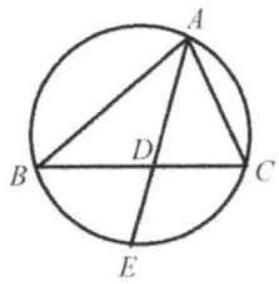
\includegraphics[width=\textwidth]{images/165(1).jpg}\\
\(\angle B=\angle E=\alpha\) (Both face the same arc \(A C\) ).\\
Since \(A D\) is the angle bisector of \(\angle A, \angle E A C=\angle B A D=\beta\).

So \(\triangle E A C \sim \triangle B A D\)\\
\(\frac{A C}{A D}=\frac{A E}{A B} \quad \Rightarrow \quad A B \times A C=A D \times A E\).\\
\centering
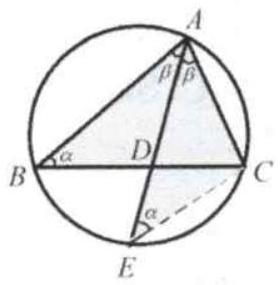
\includegraphics[width=\textwidth]{images/165.jpg}

Method 2:\\
Connect \(B E\).\\
\(\angle C=\angle E=\alpha\) (Both face the same arc \(A B)\).\\
Since \(A D\) is the angle bisector of \(\angle A, \angle D A C=\angle E A B=\beta\).\\
So \(\triangle E A B \sim \triangle C A D\)\\
\(\frac{A C}{A D}=\frac{A E}{A B} \quad \Rightarrow \quad A B \times A C=A D \times A E\).\\
\centering
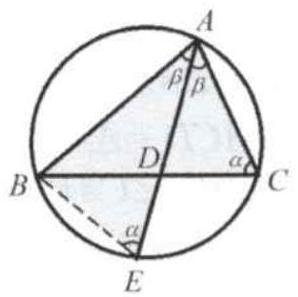
\includegraphics[width=\textwidth]{images/165(3).jpg}


\end{document}
